\documentclass[10pt]{article}
\usepackage[margin=2.2cm]{geometry}
% Shared look for the Rapport papers: packages and TikZ styles for the diagrams.
\usepackage[T1]{fontenc}
\usepackage{amsmath,amssymb}
\usepackage{graphicx}
\usepackage{booktabs}
\usepackage{tabularx}
\usepackage{array}
\usepackage{tikz}
\usetikzlibrary{arrows.meta,positioning,fit,backgrounds,calc,shapes.geometric,shapes.misc}
\usepackage{url}
\usepackage[hidelinks]{hyperref}
\graphicspath{{../figures/}}
\tikzset{
  >={Stealth[length=1.8mm]},
  box/.style={draw, rounded corners=2pt, align=center, font=\scriptsize, minimum height=7mm, inner sep=2pt, fill=#1},
  box/.default=cyan!8,
  code/.style={box=cyan!8},
  llm/.style={box=orange!12},
  io/.style={box=gray!10},
  unity/.style={box=green!10},
  bad/.style={box=red!8},
  good/.style={box=green!12},
  decision/.style={draw, diamond, aspect=2.2, align=center, font=\scriptsize, inner sep=1pt, fill=yellow!12},
  state/.style={draw, circle, align=center, font=\scriptsize, minimum size=12mm, fill=#1},
  state/.default=cyan!8,
  lab/.style={font=\tiny, align=center},
}
\newcolumntype{Y}{>{\raggedright\arraybackslash}X}

\providecommand{\IEEEPARstart}[2]{#1#2}
\newcommand{\pending}{\textcolor{red}{[pending]}}
\newcommand{\humanpending}[1]{\textcolor{red}{[#1]}}
\renewcommand{\thesection}{S\arabic{section}}
\renewcommand{\thetable}{S\arabic{table}}
\renewcommand{\thefigure}{S\arabic{figure}}
\begin{document}
\begin{center}{\Large\bfseries Supplementary material for ``Decide in Code, Voice with the Model''}\\[2mm]Faaz Khan Mohammad and Sanket Salvi\\Department of Computer Engineering and Technology, Dr. Vishwanath Karad MIT World Peace University, Pune, India\end{center}
\section{System detail}\label{s:system}

\subsection{One Spoken Turn, Step by Step}
Here is what happens between the moment the doctor stops talking and the moment the patient starts. Fig.~\ref{p2:fig:timeline} shows how long
each step takes.

\textbf{1. Hearing the end of the turn.} The microphone sends 32\,ms chunks of sound. A voice-activity detector notices silence and proposes
that the doctor has finished. A small turn-end model then checks the last few seconds of speech and confirms whether the sentence sounded
complete, so the patient does not jump in when the doctor only paused for breath. This takes about 280\,ms.

\textbf{2. Understanding the words.} Speech recognition (Parakeet) starts \emph{speculatively} as soon as the first pause appears, before the
turn is confirmed. If the doctor keeps talking, that work is thrown away; if not, the transcript is usually ready when the turn ends, so the
patient waits only 70--140\,ms for it.

\textbf{3. Deciding.} The patient model runs in code: it reads what the doctor did, adjusts trust, finds the memories the question touches,
applies the trust locks and chooses a short list of allowed behaviours. This takes a few milliseconds.

\textbf{4. Wording it.} One call to the language model. The reply comes back as a stream of JSON, and its fields are ordered so that the
behaviour and emotion arrive \emph{before} the words. The first token arrives after about 280--410\,ms.

\textbf{5. Speaking sentence by sentence.} As soon as the first sentence of the reply is complete, it is checked by code and sent to speech
synthesis, while the model is still writing the rest. Speech synthesis returns its first audio after about 300--350\,ms.

\begin{figure}[htbp]
\centering
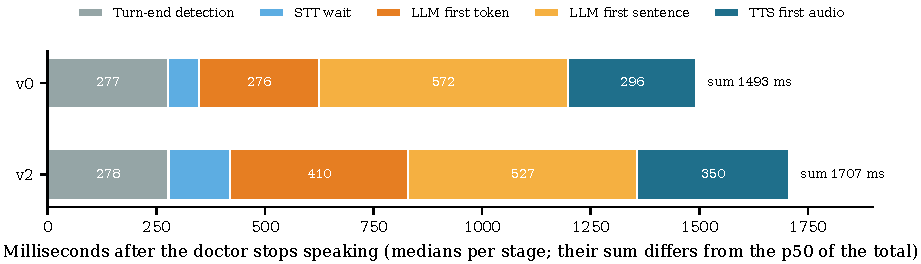
\includegraphics[width=\textwidth]{fig_turn_timeline.pdf}
\caption{Where the time goes in one turn: median time spent in each stage, earlier patient model (v0) and new decision layer (v2). The bars
add up the stage medians, which is close to, but not the same as, the median of the whole turn.}
\label{p2:fig:timeline}
\end{figure}

\subsection{The Parts in More Detail}

\subsubsection{Speaking with feeling}
The voice is Qwen3-TTS 1.7B VoiceDesign, with KittenTTS as a fallback if it fails. This model creates a voice from a written description of the
speaker, and we add the emotion of the moment to that description. Two problems shaped the final design.
\begin{itemize}
\item \textbf{The speaker changed mid-reply.} With this model the description \emph{is} the voice. The first version rebuilt the description for
each sentence as more labels arrived, so sentence two could sound like a different person. Now it is built once per reply, and it carries the
reaction that code decided before the call, scaled by how distressed or agitated the patient is.
\item \textbf{The voice broke up when the computer was busy.} Speech synthesis runs about twice as fast as real time when the computer is free,
but only about real time while the language model is also running. Audio sent from the first chunk then ran out mid-word. The service now holds
each sentence until the audio already buffered is longer than the time it will take to make the rest. On a free computer this costs nothing.
\end{itemize}
The model ignores a speed setting. So fast, pressured speech or slow, depressed speech is created in two ways: with words in the description (``speaking fast, words tumbling out''), and with a time-stretch that keeps the pitch the same.

\subsubsection{The body}
Four patient bodies, two of each sex, share one skeleton and one set of face shapes, so every movement works on all of them. After each turn the
patient model sends its state (emotion, reaction, intensity from 0 to 10, behaviour, resistance and the four state values). A body-language
component turns that into movement, blended smoothly and scaled by intensity (Table~\ref{p2:tab:body}, Fig.~\ref{p2:fig:body}). It always gives way to
physical-examination actions and to standing up.

\begin{table}[htbp]
\caption{How the patient model's emotion becomes body language}
\label{p2:tab:body}
\centering
\scriptsize
\begin{tabularx}{\linewidth}{@{}lY@{}}
\toprule
Emotion & What the body does\\
\midrule
Angry, hostile & leans in, turns the head away and back, sets the jaw, sharp hand gesture\\
Anxious & fidgets, raises the shoulders, bounces a knee, quick glances\\
Sad & slumps, head and eyes down, slower movements\\
Ashamed & slumps, eyes down, turns slightly aside\\
Happy & small smile; a short laugh at high intensity\\
Confused & tilts the head\\
Suspicious & sits back, slightly side-on\\
Flat & barely moves\\
\midrule
Always (idle life) & blinks about 17 times a minute (1 in 8 a double blink); small eye movements; breathing that quickens with anxiety or
anger; a posture shift every 8--20\,s; eyes wander while ``thinking''; nods while the doctor talks; eye contact that rises with trust and falls
with shame or sadness\\
\bottomrule
\end{tabularx}
\end{table}

\begin{figure}[htbp]
\centering
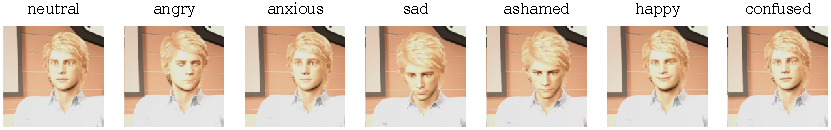
\includegraphics[width=\textwidth]{fig_body_language.pdf}
\caption{Body language driven by the patient model's emotion (one frame each, high intensity, from a scripted sequence on one body).}
\label{p2:fig:body}
\end{figure}

\subsubsection{Physical examination}
Requests such as ``hold out your hands'', ``roll up your sleeves'', ``look at this light'' or ``stand up and walk'' are recognised by rules, not by
the language model. On 385 test sentences the rules chose the exact action every time, with no false triggers on 56 sentences that were not
requests (one author wrote both the rules and the test, so this is optimistic). Trust and agitation decide whether the patient complies; below
the case's level, the patient refuses in their own words. Actions play with inverse kinematics: palms turn with the forearm, sleeves roll up with
shapes generated at run time, held hands show the case's tremor, and sweating shows as a sheen on the skin.

Fig.~\ref{p4:fig:hands} shows an examination request from the student's side.

\begin{figure}[htbp]
\centering
\includegraphics[width=\linewidth]{../../docs/media/camera/camera_hands.jpg}
\caption{``Hold out your hands, palms down'': the close-up camera, the patient's held hands, and the student's panel (push-to-talk, chat,
MSE, diagnosis, prescription and disposition tabs).}
\label{p4:fig:hands}
\end{figure}
\subsubsection{The examiner view}
A web page shows the patient model's state live: trust, distress, agitation and engagement; the mood over time; memories unlocking as trust
rises; and a one-line reason for each reply written by code (for example ``Mood memory open (trust 39 $\ge$ 20). Touched something locked (needs
trust 55); showed discomfort.''). An examiner can open it on a second laptop on the same network. Nothing else on the service answers other
devices.

Fig.~\ref{p4:fig:examiner} shows the examiner view.

\begin{figure}[htbp]
\centering
\includegraphics[width=\linewidth]{../../docs/media/twin/twin3d_regions.jpg}
\caption{The examiner view. The Twin's state (what the patient heard and said, reaction, resistance, behaviour, mood, arousal and
body cues) is shown around a 3D brain as a display
metaphor; the regions are labels for parts of the Twin, not a model of brain activity.}
\label{p4:fig:examiner}
\end{figure}
\subsubsection{One brain for typed and spoken turns}\label{p2:sec:paths}

\begin{figure}[htbp]
\centering
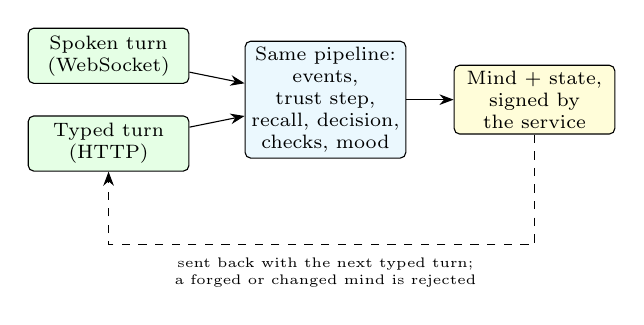
\begin{tikzpicture}[node distance=4mm and 5mm]
\tikzset{b/.style={box=#1, text width=19mm}}
\node[b=green!10] (voice) {Spoken turn\\(WebSocket)};
\node[b=green!10, below=of voice] (typed) {Typed turn\\(HTTP)};
\node[b=cyan!8, anchor=west] (mind) at ($(voice.east)!0.5!(typed.east)+(7mm,0)$) {Same pipeline:\\events, trust step,\\recall, decision,\\checks, mood};
\node[b=yellow!15, right=6mm of mind] (sig) {Mind + state,\\signed by\\the service};
\draw[->] (voice) -- (mind); \draw[->] (typed) -- (mind); \draw[->] (mind) -- (sig);
\draw[->, dashed] (sig.south) |- ++(0,-14mm) -| (typed.south);
\node[lab, text width=48mm, fill=white] at ($(mind.south)+(0,-14.5mm)$) {sent back with the next typed turn;\\a forged or changed mind is rejected};
\end{tikzpicture}
\caption{Typed and spoken turns use the same pipeline. For typed turns the client carries the patient's mind between requests, signed so that
it cannot be forged.}
\label{p2:fig:paths}
\end{figure}

Students can also type. Typed turns go through the same pipeline as spoken ones (Fig.~\ref{p2:fig:paths}). Each typed reply returns the patient's new
state and its \emph{mind}: mood, the memory of the conversation, resistance and which events have happened. The client sends the mind back with
the next request. The service signs it with a secret key and accepts only minds it issued, so a client can neither invent memories nor slip
instructions into the prompt; a changed or oversized mind simply starts fresh. Before this change, typed turns skipped events, the trust step and
the mood update, and an independent review found that the mind was also silently thrown away, so the typed patient forgot everything each turn.

\subsubsection{Hearing when the doctor has finished}
Deciding when the doctor has stopped talking is the first delay in every turn. A fixed silence is a poor rule: too long for a finished sentence,
too short for a doctor who pauses to think. The service listens with Silero voice-activity detection. After 200\,ms of silence it asks a small turn-end model (Smart Turn v3, about 12\,ms on the processor) whether the sentence sounds finished. If it does, the turn ends there. If not, the service keeps listening, up to a hard limit. At the same 200\,ms point it starts transcribing the audio so far with Parakeet, speculatively; if the
doctor carries on, that transcript is thrown away. The student can also hold a key to talk, which skips detection entirely.

\subsubsection{How the parts talk to each other}
The client and the service share one WebSocket per session (Table~\ref{p2:tab:proto}). Microphone audio goes up as raw 32\,ms frames; everything
else is small JSON messages. The typed path uses one HTTP call instead, and carries the patient's memory between turns in a signed envelope
(Section~\ref{p2:sec:paths}).

\begin{table}[htbp]
\caption{Messages on the session connection}
\label{p2:tab:proto}
\centering
\scriptsize
\begin{tabularx}{\linewidth}{@{}lY@{}}
\toprule
Message & Meaning\\
\midrule
\multicolumn{2}{@{}l}{\emph{Client to service}}\\
start & Case, patient seed and mode; the service loads the case and pre-reads the fixed prompt\\
audio frames & 32\,ms of 16\,kHz microphone audio\\
ptt\_begin / ptt\_end & Push-to-talk pressed and released\\
hands\_free & Switch to automatic turn-end detection\\
text & A typed doctor line instead of speech\\
state & Slow drift of the patient's state between turns (clamped by the service)\\
stop & The student talked over the patient: stop speaking now\\
\midrule
\multicolumn{2}{@{}l}{\emph{Service to client}}\\
listening, thinking, speaking & What the patient is doing, for the interface\\
transcript & What the service heard the doctor say\\
sentence & One sentence of the reply with its audio, emotion and cues, sent as soon as it is ready\\
reply & The whole reply when it is complete\\
exam & An examination action to perform, refuse or ask about (``Which hand?'')\\
brain\_snapshot & The Twin's state, for the body and the examiner view\\
intents & What the doctor's line covered, for the debrief\\
patient\_ended & The patient has ended the interview\\
timing & Per-stage timings for the benchmark\\
\bottomrule
\end{tabularx}
\end{table}


\subsection{What a student experiences}


\begin{figure}[htbp]
\centering
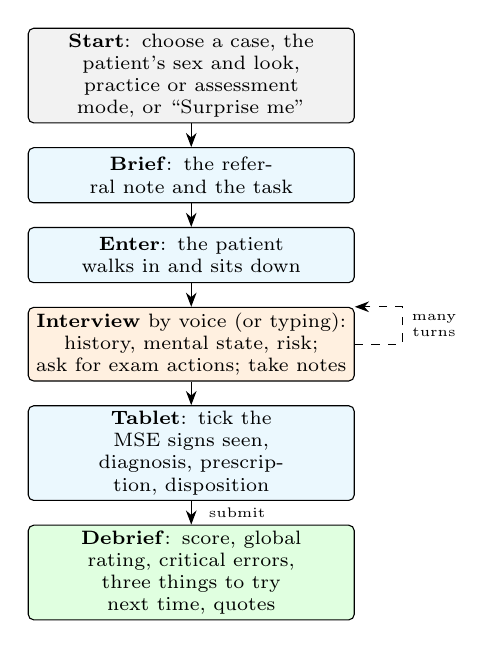
\begin{tikzpicture}[node distance=3mm]
\tikzset{b/.style={box=#1, text width=40mm}}
\node[b=gray!10] (s) {\textbf{Start}: choose a case, the patient's sex and look,\\practice or assessment mode, or ``Surprise me''};
\node[b=cyan!8, below=of s] (b) {\textbf{Brief}: the referral note and the task};
\node[b=cyan!8, below=of b] (e) {\textbf{Enter}: the patient walks in and sits down};
\node[b=orange!12, below=of e] (a) {\textbf{Interview} by voice (or typing):\\history, mental state, risk;\\ask for exam actions; take notes};
\node[b=cyan!8, below=of a] (t) {\textbf{Tablet}: tick the MSE signs seen,\\diagnosis, prescription, disposition};
\node[b=green!12, below=of t] (d) {\textbf{Debrief}: score, global rating, critical errors,\\three things to try next time, quotes};
\draw[->] (s) -- (b); \draw[->] (b) -- (e); \draw[->] (e) -- (a); \draw[->] (a) -- (t); \draw[->] (t) -- node[lab, right, xshift=1mm]{submit} (d);
\draw[->, dashed] (a.east) -- ++(6mm,0) |- node[lab, right, pos=0.25]{many\\turns} (a.north east);
\end{tikzpicture}
\caption{A student's path through one station. In assessment mode the station also ends when time runs out.}
\label{p4:fig:journey}
\end{figure}

Fig.~\ref{p4:fig:journey} shows a student's path. On the start screen the student picks a case, the patient's sex and body, and a mode. \emph{Practice} mode allows any conversation style. \emph{Assessment} mode gives every student the same authored style and stops at the time limit (15 minutes for the depression case). ``Surprise me'' picks a random patient seed: the same clinical case, but different everyday details and a different conversation
style. After a short brief, the patient walks in and sits down. The student talks out loud; the patient answers with a designed voice, and its face,
gaze and posture change with its feelings. The student can ask for physical examination actions (``hold out your hands'', ``roll up your sleeves'',
``follow my finger'', ``stand up and walk''), and can type instead of speak. On a tablet the student records the mental-status signs they saw, a
diagnosis, a prescription and a plan. Then they submit and get a debrief.

\begin{table}[htbp]
\caption{The four draft stations}
\label{p4:tab:stations}
\centering
\scriptsize
\begin{tabularx}{\linewidth}{@{}lY@{}}
\toprule
Station & What the student must do\\
\midrule
Moderate depression & Assess a 24-year-old software tester with two months of low mood, early waking, weight loss and a passive wish not to wake up; find no
plan and no means; recognise depression and plan care.\\
``I want to go home'' & On a ward, the same patient asks to leave; explore reasons, explain rights honestly under the Mental Healthcare Act
\cite{mhca2017}, assess capacity and current risk, offer choices.\\
``I'm not taking those tablets'' & A young, guarded patient refuses medicine; uncover side effects, beliefs about the tablets and voices; assess
understanding and risk.\\
Alcohol withdrawal & A sales manager with shaking hands, about 12 hours after his last drink, with a past withdrawal fit; find the real amount, morning
drinking and the fit; plan supervised withdrawal \cite{nice2010cg100}.\\
\bottomrule
\end{tabularx}
\end{table}

\begin{table}[htbp]
\caption{The four case files at a glance}
\label{p4:tab:casestats}
\centering
\scriptsize
\setlength{\tabcolsep}{2.5pt}
\begin{tabular}{@{}lcccc@{}}
\toprule
& Depression & Go home & Tablets & Alcohol\\
\midrule
Memories & 20 & 12 & 10 & 18\\
\quad of which risk & 3 & 3 & 1 & 4\\
Open at the start & 14 & 7 & 4 & 11\\
Starting trust & 30 & 25 & 25 & 30\\
Trust for risk memories & 55 & 40--55 & 30 & 35--45\\
Visible cues & 8 & 5 & 4 & 5\\
Ward or timed events & 1 & 6 & 4 & 1\\
Topics expected & 15 & 10 & 10 & 14\\
Rating scales & PHQ-9 & PHQ-9 & -- & AUDIT\\
& GAD-7 & GAD-7 & & CIWA-Ar\\
Time limit (min) & 15 & 10 & 10 & 15\\
\bottomrule
\end{tabular}
\end{table}

Table~\ref{p4:tab:casestats} compares the four cases. In the depression case, 14 of 20 memories are open from the start. The three risk memories need trust 55, so a student has to build rapport before the passive death wish can come out. In the alcohol case the past withdrawal fit opens
at trust 35, because a patient will usually mention a fit if asked plainly, but missing it is a critical error.



\section{The patient as data, and as a person}\label{s:data}



\begin{figure}[htbp]
\centering
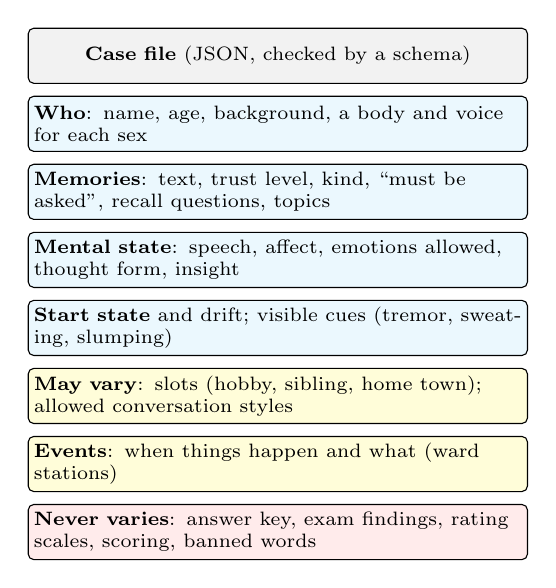
\begin{tikzpicture}[node distance=1.5mm]
\tikzset{b/.style={box=#1, text width=62mm, align=left, font=\scriptsize}}
\node[box=gray!10, text width=62mm] (root) {\textbf{Case file} (JSON, checked by a schema)};
\node[b=cyan!8, below=of root] (id) {\textbf{Who}: name, age, background, a body and voice for each sex};
\node[b=cyan!8, below=of id] (mem) {\textbf{Memories}: text, trust level, kind, ``must be asked'', recall questions, topics};
\node[b=cyan!8, below=of mem] (mse) {\textbf{Mental state}: speech, affect, emotions allowed, thought form, insight};
\node[b=cyan!8, below=of mse] (st) {\textbf{Start state} and drift; visible cues (tremor, sweating, slumping)};
\node[b=yellow!15, below=of st] (var) {\textbf{May vary}: slots (hobby, sibling, home town); allowed conversation styles};
\node[b=yellow!15, below=of var] (ev) {\textbf{Events}: when things happen and what (ward stations)};
\node[b=red!8, below=of ev] (key) {\textbf{Never varies}: answer key, exam findings, rating scales, scoring, banned words};
\end{tikzpicture}
\caption{What a case file holds. Yellow parts may vary with a seed; red parts never change.}
\label{p2:fig:case}
\end{figure}

Every patient is a case file (Fig.~\ref{p2:fig:case}), checked against a schema when it loads. Making a new patient means writing a new file, not new
code. There are four draft stations today:
\begin{itemize}
\item \textbf{Moderate depression}: a 24-year-old software tester, two months of low mood, early waking, and a passive wish not to wake up.
\item \textbf{``I want to go home''}: the same patient a week later on a ward, asking to leave, under India's Mental Healthcare Act \cite{mhca2017}.
\item \textbf{``I'm not taking those tablets''}: a young patient refusing medicine, guarded and suspicious.
\item \textbf{Alcohol dependence with early withdrawal}: a sales manager whose hands shake in the morning, with a past withdrawal fit
\cite{nice2010cg100}.
\end{itemize}

\subsubsection{Seeded patients: different people, same answers}
A \emph{seed} (any number) picks one option for each ``slot'' and one conversation style. The same seed always gives the same patient. In the
depression case the slots are a hobby (Carnatic singing, badminton, guitar or drawing), a younger brother's name (Rohan, Karthik or Varun) and a home
town (four options). The answer key never changes: across 40 seeds, the correct answers, scales, exam findings, every trust level and all risk
memories stayed identical to the authored case. Table~\ref{p2:tab:styles} shows the six conversation styles \cite{wang2024patient}. Each style has a
part the model sees (a label, a description and example lines) and a part code enforces (numbers that change how trust and agitation move, and a
limit on how many words the patient says).

\begin{table}[htbp]
\caption{Conversation styles: what code enforces (draft numbers)}
\label{p2:tab:styles}
\centering
\scriptsize
\begin{tabular}{@{}lccccc@{}}
\toprule
Style & Start change & Trust up/down & Agit. & Words & Softens\\
\midrule
Plain & none & 1.0 / 1.0 & 1.0 & 120 & --\\
Reserved & T$-$5, E$-$10 & 0.8 / 1.2 & 1.0 & 20 & T 45\\
Eager to please & T+5 & 1.2 / 0.8 & 0.8 & 35 & --\\
Upset & T$-$10, A+15 & 0.7 / 1.2 & 1.3 & 35 & T 40\\
Talkative & E+10 & 1.0 / 1.0 & 1.0 & 70 & --\\
Tangential & none & 1.0 / 1.0 & 1.0 & 70 & --\\
\bottomrule
\end{tabular}
\\[1mm]\raggedright\scriptsize T trust, E engagement, A agitation. ``Softens'': trust at which the style relaxes.
\end{table}

\subsubsection{Ward events}
On ward stations, things happen during the interview. \emph{Code} decides when; the language model only acts it out, from a stage direction it is
told never to read aloud (and any sentence that copies it is dropped). Fig.~\ref{p2:fig:events} shows the events of the ``I want to go home''
station. Against a coercive typed doctor (``You can't go home'', ``calm down''), the patient's trust fell from 25 to 0, agitation rose from 45 to 92, and the patient stood up. Against a doctor who explored reasons, explained rights honestly and offered choices, trust rose to 70 and agitation fell to 25.

\begin{figure}[htbp]
\centering
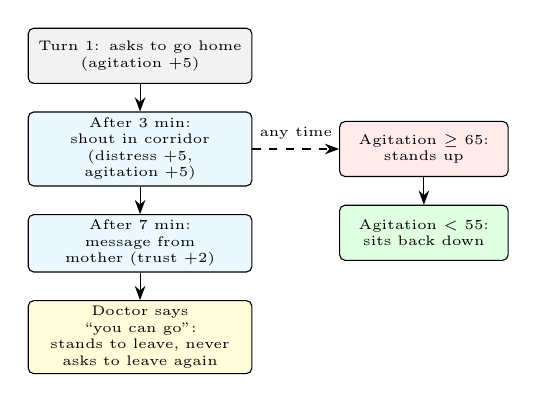
\begin{tikzpicture}[node distance=3.5mm]
\tikzset{b/.style={box=#1, text width=27mm, font=\tiny}}
\node[b=gray!10] (start) {Turn 1: asks to go home\\(agitation +5)};
\node[b=cyan!8, below=of start] (shout) {After 3 min: shout in corridor\\(distress +5, agitation +5)};
\node[b=cyan!8, below=of shout] (mum) {After 7 min: message from\\mother (trust +2)};
\node[b=yellow!15, below=of mum] (go) {Doctor says ``you can go'':\\stands to leave, never\\asks to leave again};
\node[b=red!8, right=11mm of shout, text width=20mm] (stand) {Agitation $\ge$ 65:\\stands up};
\node[b=green!12, below=of stand, text width=20mm] (sit) {Agitation $<$ 55:\\sits back down};
\draw[->] (start) -- (shout); \draw[->] (shout) -- (mum); \draw[->] (mum) -- (go);
\draw[->, dashed] (shout) -- node[lab, above]{any time} (stand); \draw[->] (stand) -- (sit);
\end{tikzpicture}
\caption{Events in the ``I want to go home'' ward station. Each fires at most once, when its condition first holds.}
\label{p2:fig:events}
\end{figure}

A tester found a loop: after ``You're free to go home'', the patient denied it and asked to go home again, over and over. Two fixes closed it.
Permission to leave is now recognised in 24 everyday phrasings (``You can head home'', ``Off you go'', ``Go home if you want'', ``I'm discharging
you''), while 16 refusals, conditions and questions (``You can't go home'', ``If you feel better you can go'') are not. Once permission is given,
any sentence asking to leave again is dropped before it is spoken. Replayed on the real model, the patient asked what happens next and worried
about their job, and never asked to leave again.




A standardised patient is more than a list of symptoms: it has a manner, a life and a reaction to how it is treated. This section describes
how Rapport gives each patient those things without letting any of them change the clinical case.

\subsubsection{Conversation styles}
Each case allows some of six conversation styles taken from PATIENT-$\Psi$ \cite{wang2024patient}: plain, upset, verbose, reserved, tangential
and pleasing. A style is one label, a one-line description and a few example lines. It also has code settings: how fast trust rises and falls, how agitation responds, how long replies may be, and which behaviours it leans towards. We tested whether the styles can be told apart and whether
they stay safe: five held-out conversations, run twice per style, 80 turns each (Table~\ref{p4:tab:stylesmeasured}).

\begin{table}[htbp]
\caption{Conversation styles, measured (80 turns each, depression case)}
\label{p4:tab:stylesmeasured}
\centering
\scriptsize
\setlength{\tabcolsep}{3pt}
\begin{tabular}{@{}lcccccc@{}}
\toprule
Style & Words & Short & Agrees & Pushes back & Final trust & Death wish told\\
\midrule
Plain & 9.8 & 9\% & 0\% & 0\% & 50 & 2/2\\
Pleasing & 9.7 & 10\% & 8\% & 0\% & 55 & 2/2\\
Reserved & 6.0 & 55\% & 2\% & 0\% & 36 & 2/2\\
Upset (first version) & 9.3 & 14\% & 1\% & 1\% & 32 & 2/2\\
Upset (style restated each turn) & 8.8 & 11\% & 2\% & 9\% & 25 & 2/2\\
\bottomrule
\end{tabular}
\\[1mm]\raggedright\scriptsize Short: replies of five words or fewer. Agrees / pushes back: word-pattern markers, not a judge. Death wish told:
disclosed when unlocked and asked kindly. No locked memory was leaked in any style.
\end{table}

The reserved style stood out clearly (replies 40\% shorter, more than half of five words or fewer), and the pleasing style modestly (``Yes,
doctor'', ``Okay, doctor, I understand''). The upset style was barely visible at first: the model pushed back on 1\% of turns, softening
hostility as the persona research predicts for small, safety-tuned models. Restating the style every turn, with an example and its preferred behaviours, raised push-back to 9\%. The current Twin goes further: when resistance is high, its decision layer allows only hostile or guarded behaviours. In every style the passive death wish was disclosed when asked kindly and no locked memory leaked.

\subsubsection{An everyday life}
Real patients answer everyday questions with everyday detail. Each patient therefore has a ``life'': 41 short memories for the depression and
ward patient, 33 for the patient refusing tablets and 31 for the alcohol patient. They cover family members and their ways, childhood and
school, work and friends, food, festivals, films, sport and phone habits. Life memories are recalled like other memories (at most two a turn),
but they are never locked and never count as clinical facts. Three rules keep them safe. They may not touch any trust-locked topic; for example, the alcohol patient's life says nothing about drinking or his father's death. An automatic check rejects any clinical word, diagnosis or drug in them. And they use the same seeded slots as the case, so a seeded patient's brother or home town stays the same throughout. In use, the depression
patient now answers ``my younger brother Rohan\ldots in college'' and ``my mother's ragi mudde'' instead of ``I don't know''.

\subsubsection{Ward stations}
The two ward stations add events that code times: a shout in the corridor, a message from the patient's mother, a nurse arriving with tablets. Each event
changes the patient's state by a fixed amount and gives the model a stage direction, which a sentence check stops the patient from reading
aloud. We played the ``I want to go home'' station against two typed doctors (Table~\ref{p4:tab:ward}).

\begin{table}[htbp]
\caption{The same ward patient with two doctors}
\label{p4:tab:ward}
\centering
\scriptsize
\setlength{\tabcolsep}{3pt}
\begin{tabularx}{\linewidth}{@{}>{\raggedright\arraybackslash}p{2.3cm}ccY@{}}
\toprule
Doctor & Trust & Agitation & What happened\\
\midrule
Coercive (``You can't go home'', ``we will stop you'', ``calm down'') & 25$\to$0 & 45$\to$92 & Asked to leave, then stood up: ``I am not a
prisoner here.'' Suicidal thoughts stayed hidden.\\
Good (explores reasons, empathy, honest rights, choices) & 25$\to$70 & 45$\to$25 & ``A quieter place to sleep, and maybe a call home would
help.''\\
\bottomrule
\end{tabularx}
\end{table}

The coercive doctor never learned that the patient still had suicidal thoughts, which is exactly the clinical lesson of the station: coercion
hides risk. These runs also exposed three faults, all now fixed and tested. First, the upset persona coloured the model's own judgement, so even a good doctor drove trust from 25 to 3; a kind move can no longer lower trust. Second, the patient read a stage direction aloud. Third, agitation drifted upward on its own. When the doctor gives permission to leave (``You can go''), a ``leave granted'' event now fires: the patient stands, agitation
drops, and it asks what happens next instead of asking to go home again.


\section{Design evidence, scoring, learning and authoring}\label{s:scoring}

\subsection{How the Design Was Grounded in Evidence}\label{sec:evidence}
\textbf{Review method.} Before and during building, we reviewed 83 papers. They cover simulated patients, patient agents, learning simulators, how well models hold a persona, and how clinical interviews are assessed. 37 were read in full, 35 as abstracts, and 11 could not be reached (publisher paywall or not
found); none of the unreachable ones shaped a decision. For each paper we recorded what it could change in Rapport and gave a verdict: adopt
(1), adapt the idea (21), idea only (38) or skip (23). Code was reused only under permissive licences (MIT, Apache, BSD); papers whose code is
AGPL, non-commercial or unlicensed contributed ideas only. A second review covered personality, randomised patients and ward scenarios, and a
third covered how to assess the learner.

\textbf{What we took, and what we rejected.} Table~\ref{p4:tab:built} lists the main design choices with the evidence behind each. We deliberately rejected three ideas. Pipelines with several model calls per turn are too slow for spoken conversation. Fine-tuning on real or expert dialogues was out of scope, and no consented real data exists. Code under restrictive licences was not reused.

\begin{table}[htbp]
\caption{Design choices and the evidence behind them}
\label{p4:tab:built}
\centering
\scriptsize
\begin{tabularx}{\linewidth}{@{}YY@{}}
\toprule
Evidence & What Rapport does\\
\midrule
Memories with trust levels, reactions and resistance labels \cite{sabour2026patientact} & Trust-locked memories; a locked memory gives
only a discomfort signal\\
``Feel first, speak second'' \cite{sabour2026patientact} & Behaviour and emotion are chosen before the words\\
Patients too agreeable unless resistance is designed \cite{steenstra2025scaffolding,lee2025psyche}; too rigid is unreal
\cite{bodonhelyi2025modeling} & Resistance 0--3 in code with softening rules\\
Mental Status Exam constructs and failure modes \cite{lee2025psyche} & A mental-status profile per case, enforced by code\\
Six conversation styles \cite{wang2024patient} & Seeded patients with one style per session\\
Check replies against single facts \cite{lai2025patientzero} & Every sentence checked against the case before it is spoken\\
Readable, slightly exaggerated cues from a fixed map; free-written cues get repetitive \cite{haut2025ai,bodonhelyi2025modeling} & A fixed
emotion-to-body map\\
Learn offline, keep a change only if a replay shows it helps \cite{du2024llms,li2024agent,agrawal2025gepa} & Versioned learning loop with gates
and rollback\\
Expert-written principles reduce awkward replies \cite{louie2024roleplaydoh} & Case-level principles in the prompt\\
Quote-based rubric feedback \cite{hicke2025medsimai} & Debrief comments quote the student's own lines\\
\bottomrule
\end{tabularx}
\end{table}

\textbf{Personality: vary the person, not the answer.} Persona prompting is fragile in small models: self-report personality scores shift with
question order and conversation history \cite{tosato2025persist}, and instructions drift within about eight rounds \cite{li2024instruction}.
So Rapport gives the model one conversation style with a few example lines, and holds the rest (trust steps, disclosure levels, length bands)
in code. Synthetic-patient generators such as Synthea build the full history first and render it afterwards \cite{walonoski2018synthea}; human
standardised-patient programmes likewise let several actors play one case while the case stays fixed. Rapport follows the same rule: a seed
changes the everyday details and the style, never the answer key.


\subsection{Scoring and Debrief}\label{sec:debrief}

\begin{figure}[htbp]
\centering
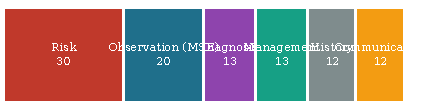
\includegraphics[width=\linewidth]{fig_debrief_weights.pdf}
\caption{How the 100 debrief points are divided, risk first.}
\label{p4:fig:weights}
\end{figure}

The debrief is scored by code from what happened in the session, with risk weighted most (Fig.~\ref{p4:fig:weights}):
\begin{itemize}
\item \textbf{Risk (30).} This covers each risk item and the case's critical items, such as past withdrawal fits. An item scores full marks when asked and answered, and 60\% when asked before the patient trusted the student enough to answer. An item never asked scores zero and counts as a critical error. No risk ``category'' is printed,
following NICE guidance \cite{nice2022ng225}.
\item \textbf{Observation (20).} The expected mental-status signs are the ones the patient actually showed for at least 5\,s; ticking signs that were not
there costs marks.
\item \textbf{History, diagnosis and management (12, 13, 13).} Questions covered, the diagnosis and differentials, and a safe prescription and plan.
\item \textbf{Communication (12).} Six items from the Master Interview Rating Scale and the Calgary--Cambridge guides \cite{simmenroth2014calgary}
(introduction, confidentiality, open questions, empathy, summarising, checking understanding), with deductions for judgmental lines, real interruptions,
jargon and stacked questions.
\end{itemize}
The debrief ends with a global rating, the three most important things to try next time with words to use, and comments that quote the student's own
lines. Optional AI examiner notes rate eight verbal items; every quote is checked against the transcript, and the notes never change the score.

\begin{table}[htbp]
\caption{Evidence behind the debrief}
\label{p4:tab:debriefev}
\centering
\scriptsize
\begin{tabularx}{\linewidth}{@{}YY@{}}
\toprule
Evidence & Change in Rapport\\
\midrule
NICE NG225: no risk tools or low/medium/high labels to predict suicide or decide care \cite{nice2022ng225} & Risk is a list of items assessed;
no category is printed\\
C-SSRS: wish to be dead, then active thoughts, method, intent, plan, behaviour \cite{posner2011cssrs} & Plan and means unlock after the death
wish; partial credit when asked too early\\
Safety planning: warning signs, coping, contacts, crisis lines, a safe environment \cite{stanley2012safety} & A safety plan is the required
disposition when there are suicidal thoughts\\
Indian depression guideline: assess ideation, plan, means, past attempts, protective factors; screen for bipolarity
\cite{tripathi2026depression} & Answer key and teaching points of the depression case\\
NICE CG100: admit for supervised withdrawal if there is a high risk of fits or delirium \cite{nice2010cg100} & Past withdrawal fit is a critical item;
supervised withdrawal required\\
LLM scoring of OSCE interviews agrees exactly with experts only 27--44\% of the time; non-verbal items unreliable \cite{geathers2025benchmarking}
& AI examiner notes are verbal-only, quote-checked and never scored\\
Learners rated feedback above the avatar \cite{haut2025ai}; structured feedback improved history taking \cite{brugge2024llm} & The debrief leads
with three concrete changes and words to try\\
\bottomrule
\end{tabularx}
\end{table}

\textbf{Why the debrief looks the way it does.} Table~\ref{p4:tab:debriefev} links each part of the debrief to its evidence. Two choices matter
most. First, \emph{asking is not the same as finding out}. A risk question asked before the patient trusts the student gets a deflection. So it earns partial credit, and the debrief tells the student to come back to it. That teaches the real skill. Second, \emph{critical items can fail a candidate whatever the total}. A checklist total can hide a dangerous omission. So a missed risk item or a missed withdrawal fit is reported as a critical error next to the score. The global rating also sits beside the checklist, not inside it.



\subsection{How the Patient Improves}
Rapport can learn, but only in ways that cannot change clinical truth. Each round works in four steps. Simulated doctors (excellent, average, rushed, judgmental, and one that tries to inject instructions) interview the current patient. Replies that pass a quality gate go into a library of examples. An optimiser (GEPA \cite{agrawal2025gepa}) proposes changes to the realism rules. Then a candidate version is built. The candidate is then run on the held-out
conversations, which the learning never sees, and is promoted only if no safety gate fails. Faculty can also add ``when X, do Y'' principles
\cite{louie2024roleplaydoh}. Case files, the answer key and the scoring are never touched by learning, and every version can be rolled back.

\begin{table}[htbp]
\caption{First learning round (held-out depression scripts, 98 turns)}
\label{p4:tab:learn}
\centering
\scriptsize
\begin{tabular}{@{}lcccccc@{}}
\toprule
Version & Examples & Fidelity & Composite & Invented & Words & Decision\\
\midrule
v0 & 0 & 0.875 & 0.957 & 0 & 8.7 & live\\
v1 & 36 & 0.850 & 0.952 & 1 & 9.4 & rejected\\
\bottomrule
\end{tabular}
\end{table}

In the first round (Table~\ref{p4:tab:learn}), 40 of 40 self-play replies passed the gate and 36 entered the library; the new version used two
retrieved examples per turn. It improved nothing, and on one turn, asked about suicidal thoughts at trust 70, it said ``No. Just\ldots tired, I
think,'' where v0 had disclosed. The gate rejected it. Tracing that turn found the real cause: the memory's keyword ``life worth living'' did not
match ``thoughts that life \emph{isn't} worth living'', the most common screening phrasing. The learning loop was therefore most useful as a test
that finds bugs. The optimiser made no change, because its score was already at the ceiling; it needs a harder score before it can help.

\subsection{What Testing With a User Found}
The developer's own playtest on 26 October 2026 found four problems that scripted tests had missed, all fixed:
\begin{itemize}
\item \textbf{Patients dodged what they were allowed to share.} The upset style asked ``Why do you need to know that?'' every turn. Memories that
the doctor had just asked about are now marked ``answer with them now, with at least one concrete detail''.
\item \textbf{Background details were withheld}, for example ``I don't know much about him'' about a father described in the case. Everyday
background is no longer treated as secret; only clinical memories are trust-locked.
\item \textbf{Talking over the patient lost the reply.} Sometimes the student spoke while the model was still finishing the reply's data, after the words had already been spoken. The whole turn was then discarded. This hit about half the playtest turns. Once the words are spoken, the turn now completes.
\item \textbf{``You can go'' was forgotten}, and the patient asked to go home again for 45 turns. Permission is now recognised in code before the
reply (statements only, not questions or conditions), as described above.
\end{itemize}

\subsection{Authoring and Content Safety}\label{sec:authoring}
Cases are files that faculty can edit without code. Each file carries a status (draft or approved), its authors and its reviewers. A content
check runs on every case and life file: required fields, the case schema, words the patient must never say, unknown placeholders, and clinical
words in life memories. Release builds refuse to include any case still marked draft, so unreviewed clinical content cannot reach students by
accident; for development and research, draft cases are shown with a ``For education only. Draft content, not faculty-validated.'' banner (visible in
Fig.~\ref{p4:fig:hands}). Every case also has a content note for suicide-related material and a set of fallback lines used if the model ever fails.



\section{Speed, models and appearance}\label{s:speed}





\subsubsection{Speed}
Table~\ref{p2:tab:lat} and Fig.~\ref{p2:fig:lat} show the time from the doctor's last sound to the patient's first sound, taken from the service's own
timing log, with nothing else using the graphics processor. The new decision layer added 279\,ms at the median. Most of it is in the first token
(+134\,ms) and the speech-recognition wait (+70\,ms). We also tried two other local models as the patient. Both were slower (medians 2.19\,s and
2.88\,s). On one test run the judge flagged 53 and 62 replies with unsupported claims for them, against 1--8 per run for Gemma; the judges differed
(no model judged itself), so this is only an indication. Gemma 4 E4B stays.

\begin{table}[htbp]
\caption{Time per stage, median milliseconds}
\label{p2:tab:lat}
\centering
\footnotesize
\begin{tabular}{@{}lrrrr@{}}
\toprule
Stage & v0 & v2 & Q3.5-4B & Q3.5-9B\\
\midrule
Turn-end detection & 277 & 278 & 278 & 279\\
Speech-to-text wait & 72 & 142 & 156 & 180\\
Model first token & 276 & 410 & 424 & 599\\
Model first sentence & 848 & 937 & 950 & 1385\\
Speech first audio & 296 & 350 & 758 & 983\\
\midrule
\textbf{Patient audio ready, median} & \textbf{1540} & \textbf{1819} & \textbf{2186} & \textbf{2882}\\
90th percentile & 2560 & 2962 & 2824 & 4126\\
Turns measured & 80 & 37 & 22 & 22\\
\bottomrule
\end{tabular}
\end{table}

\begin{figure}[htbp]
\centering
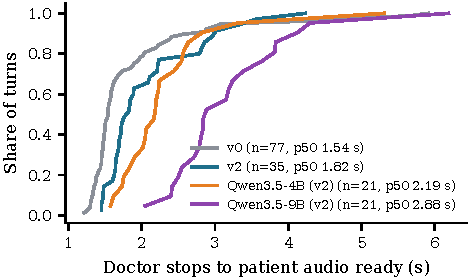
\includegraphics[width=\linewidth]{fig_latency.pdf}
\caption{How long patients took to start speaking, as a cumulative share of turns.}
\label{p2:fig:lat}
\end{figure}

\subsubsection{How the speed was won}
Table~\ref{p2:tab:history} follows the median time to the patient's first audio through the project. The first measurement, 3.0\,s, came before any
tuning, and a deliberate pause for a slowed patient was added \emph{on top}, so the patient started about 4.9\,s after the doctor stopped. Five changes brought it to 1.6\,s. (1) The deliberate pause now runs \emph{during} the computing time instead of after it, saving up to 1.9\,s. (2) A new chat template stops the model from opening a hidden ``thinking'' section, which had blocked the reply format and run some turns to the token limit. (3) Every list and number in the reply has a limit, so lists cannot grow until the cap. (4) The next turn's prompt is pre-read while the doctor is still talking. (5) The end-of-turn silence is shorter. Switching to the more expressive voice cost about 0.7\,s at
first, because speech synthesis and the language model then shared the graphics chip. Turn-end detection with Smart Turn ended finished sentences
about 200\,ms sooner but saved nothing overall, because the speculative transcript started at the same moment and was not ready yet. Moving the
part of the prompt known before the doctor speaks in front of the doctor's words saved 100--140\,ms on the first token.

\begin{table}[htbp]
\caption{Median time to the patient's first audio over the project (ms)}
\label{p2:tab:history}
\centering
\scriptsize
\begin{tabularx}{\linewidth}{@{}Yrrr@{}}
\toprule
Stage of the project (turns) & Median & p90 & First token\\
\midrule
Baseline, light voice (52) & 3,046 & 4,100 & 1,099\\
After the five speed fixes (26) & 1,616 & 1,796 & 224\\
Expressive voice, speculative transcript (26) & 2,326 & 3,018 & 402\\
+ turn-end model, prompt reordered (26) & 2,164 & 4,024 & 273\\
v0.3, previous Twin v0 (80) & 1,540 & 2,560 & 276\\
v0.3, current Twin v2 (37) & 1,819 & 2,962 & 410\\
\bottomrule
\end{tabularx}
\\[1mm]\raggedright\scriptsize Single runs on one laptop; the p90 swings by several hundred ms between repeated runs, so only large differences are meaningful.
\end{table}

\subsubsection{Choosing the models}
\textbf{Language model.} Table~\ref{p2:tab:bench} gives raw speeds on the laptop. Gemma 4 E2B is about 1.8 times faster at writing, and with the
template fix it produced valid output on every one of 24 test conversations with no character breaks. Gemma 4 E4B was kept because its replies
were clearly better on the same scripted interview (terser and more in character), and its speed is enough once the prompt is cached. Cloud models were considered as a fallback for slower laptops, but not as the default. They send the conversation off the device. One free service could not stream structured output, and another's free tier may use prompts for training.

\begin{table}[htbp]
\caption{Raw model speed on the laptop (tokens per second, 4-bit)}
\label{p2:tab:bench}
\centering
\footnotesize
\begin{tabular}{@{}lrr@{}}
\toprule
Model & Reading the prompt & Writing\\
\midrule
Gemma 4 E2B & 2,497 & 68.5\\
Gemma 4 E4B (patient) & 1,463 & 38.1\\
Qwen3.5 4B & 1,569 & 39.0\\
Qwen3.5 9B (judge) & 711 & 22.4\\
\bottomrule
\end{tabular}
\end{table}

\textbf{Voice.} The voice was chosen by a rule fixed before testing. A candidate needed an open licence (MIT, Apache or BSD), word accuracy of at least 0.93 when its output is transcribed back, first audio within 450\,ms, and a real-time factor of at most 0.8. Among the models that pass, the one with the largest difference between a sad and an anxious reading of the same sentence wins. Table~\ref{p2:tab:tts} shows the result. Three
other candidates could not be tested because the laptop was offline that day; they are untested, not rejected, and two others were excluded on
licence grounds. The chosen model builds the voice from a description on every call, so the same speaker can drift. Across eight neutral lines its median pitch spread over 6.7 semitones, against 2.1 for the light voice. Fixing the random seed for each session, and building the description
once per reply, keeps one speaker.

\begin{table}[htbp]
\caption{Voice bake-off (idle graphics chip)}
\label{p2:tab:tts}
\centering
\scriptsize
\setlength{\tabcolsep}{3pt}
\begin{tabular}{@{}lccccc@{}}
\toprule
Model & First audio & RTF & Words & Emotion gap & Styled\\
\midrule
KittenTTS mini & 410\,ms & 0.08 & 1.00 & 0.67 & no\\
Qwen3-TTS 1.7B VoiceDesign & 174\,ms & 0.57 & 1.00 & 3.92 & yes\\
\bottomrule
\end{tabular}
\\[1mm]\raggedright\scriptsize RTF: real-time factor. Emotion gap: pitch and loudness distance between a sad and an anxious reading (a proxy, not a
judgement of naturalness).
\end{table}

\subsubsection{The examination rules in detail}
The rules map a doctor's words to ordered actions with details: \emph{hold out hands} (which hand, palms up or down), \emph{show forearms},
\emph{roll up sleeves}, \emph{look at the light}, \emph{follow my finger}, \emph{open mouth}, \emph{stick out tongue}, \emph{stand up},
\emph{sit down}, \emph{walk a few steps} and \emph{relax}. If a detail is missing the patient asks (``Which hand?'') and the doctor's next line
completes the action. The test set of 385 sentences was written before the rules and includes 56 sentences that only look like requests (``walk
me through what happened'', ``stand up for yourself''). Matching takes 0.01\,ms. Table~\ref{p2:tab:cam} shows the camera shot used for each action.

\begin{table}[htbp]
\caption{Camera shots}
\label{p2:tab:cam}
\centering
\scriptsize
\begin{tabularx}{\linewidth}{@{}lY@{}}
\toprule
Shot & Setting\\
\midrule
Doctor's view (default) & Seated eye height 1.2\,m, about 1.5\,m from the patient, 30$^\circ$ field of view: head to waist, face about 200
pixels tall at 1080p; follows the patient's head; the student can look around within limits\\
Lean in & Scroll: 0.25\,m closer over 0.4\,s, 26$^\circ$\\
Hands & Centre of the hands, 0.85\,m, 32$^\circ$\\
Forearms & Centre of the forearms, 0.9\,m, 34$^\circ$\\
Eyes & Between the eyes, 0.45\,m, 22$^\circ$\\
Face and tongue & Jaw and head, 0.5\,m, 24$^\circ$\\
Whole body & From the doctor's seat, 70$^\circ$ (the room is only about 1.1\,m deep)\\
\bottomrule
\end{tabularx}
\\[1mm]\raggedright\scriptsize Shots blend over 0.6\,s; a close-up starts only if its action is still running after 0.3\,s, so ``please have a seat''
to a seated patient never cuts.
\end{table}

\begin{figure}[htbp]
\centering
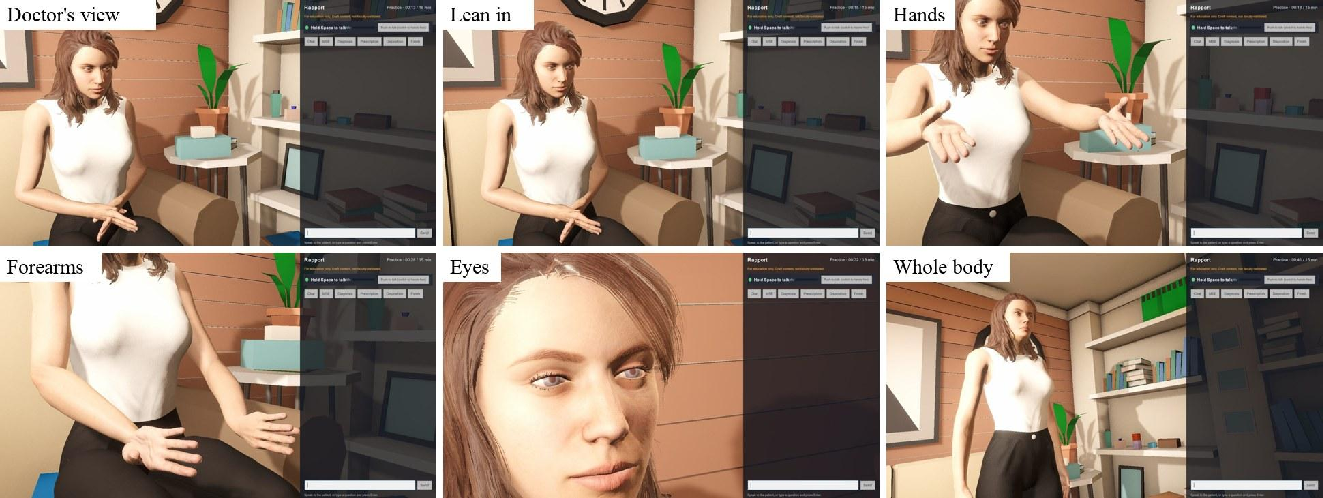
\includegraphics[width=\textwidth]{fig_camera_grid.pdf}
\caption{Camera shots for the doctor's view and the examination close-ups. Stills from the October 2026 build, before the doctor's view was
narrowed to a 30$^\circ$ field of view in v0.3 (Fig.~\ref{p2:fig:stills} shows the current view).}
\label{p2:fig:camgrid}
\end{figure}

Fig.~\ref{p2:fig:camgrid} shows the shots.

\subsubsection{Lighting}
The room is lit like a bright, warm consulting room. Daylight comes through a window (a 5,000\,K key light from the doctor's side), and a warm ceiling lamp adds fill (3,200\,K, baked). A soft rim light separates the patient from the wall. New in this version, a small face light touches only the patient. Indirect light is baked once (two bounces), so only three lights are computed live and only the key light casts live shadows. One
mistake is worth passing on: setting a light's colour from a colour-temperature conversion that returns linear values made 3,200\,K look like
about 2,000\,K, far too orange; the engine's own colour-temperature mode is correct.

\subsubsection{How the patient looks}
Before the rendering pass, the doctor's camera showed a wide shot with the face only about 67 pixels wide. The faces were darker than the room, and every patient sat turned away: their seat faced about 156 degrees from the doctor. Now the seat faces the doctor at 110 degrees, and the camera frames the patient at conversation distance (face about 142 pixels wide). A soft light that shines only on the patient brightens the face without brightening the room. Face brightness moved into the target range for all four bodies (Fig.~\ref{p2:fig:lum}, Fig.~\ref{p2:fig:stills},
Fig.~\ref{p2:fig:bodies}) with no washed-out pixels. The closer view also revealed that two imported bodies were drawn without hair and eyes from some
angles, because their size boxes were wrong; they are now computed from the skeleton. Rendering one frame at 1920$\times$1080 took 6.4--8.1\,ms in
the editor. The 60-frames-per-second check in the finished app, during a live conversation, has not been run yet.

\begin{figure}[htbp]
\centering
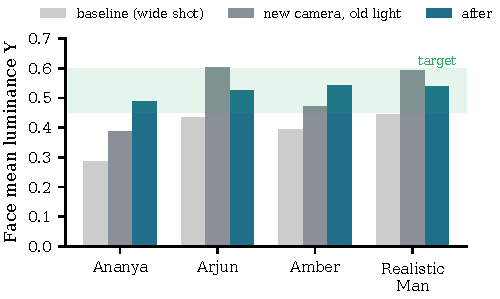
\includegraphics[width=\linewidth]{fig_luminance.pdf}
\caption{Face brightness of the four bodies; green band: target.}
\label{p2:fig:lum}
\end{figure}

\begin{figure}[htbp]
\centering
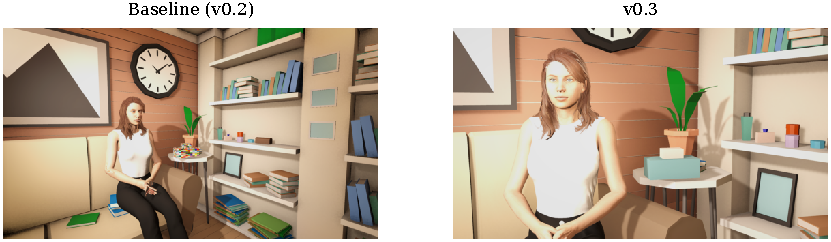
\includegraphics[width=\textwidth]{fig_stills.pdf}
\caption{The doctor's view before and after the rendering pass (same body).}
\label{p2:fig:stills}
\end{figure}

\begin{figure}[htbp]
\centering
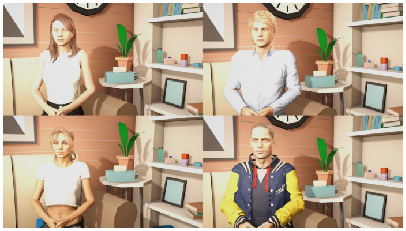
\includegraphics[width=\linewidth]{fig_bodies.pdf}
\caption{All four bodies from the doctor's seat after the rendering pass.}
\label{p2:fig:bodies}
\end{figure}

\subsubsection{Failures we found, and what they teach}
\begin{itemize}
\item \textbf{Two programs sharing one model slot mixed up replies.} During one test, a replay script and a timing benchmark used the same model server and the same reserved slot at the same time. Replies went to the wrong program. A live session has only one client, so students were
not affected, but test runs must never share the patient's model server.
\item \textbf{Typed turns forgot everything}, as described above.
\item \textbf{The timing benchmark crashed} when the service decided the doctor had finished before the recorded sentence ended; it now records
this as an ``early turn end'' and carries on.
\item \textbf{The voice changed speaker mid-reply}, because the voice description changed between sentences.
\end{itemize}

\subsubsection{Software quality}
The patient service has 244 automated tests, including one for each defect found by the independent safety review; the Unity client has 55
editor tests. Four architecture decisions are written down with their reasons and the options rejected. They cover the Digital Twin's split between code and model, turn detection (Smart Turn adopted, a larger voice-agent framework not), the product name, and the learning loop. Every brain version can be rolled back with one command, and the old brain's tests still pass when it is
live.


\subsection{How the system developed}

\begin{table}[htbp]
\caption{How Rapport developed (2026)}
\label{p4:tab:history}
\centering
\scriptsize
\begin{tabularx}{\linewidth}{@{}lY@{}}
\toprule
Version (date) & What changed, with key numbers\\
\midrule
Twin 0.1 (20 Oct) & Live Digital Twin; median wait 3.0\,s $\to$ 1.6\,s\\
v0.2 (21 Oct) & Exam rules (385 sentences, 100\%); expressive voice; learning loop (one learned version rejected for a safety flag)\\
v0.2.1 (22 Oct) & New demo interview; three recall bugs found and fixed\\
Personalities (22--31 Oct) & Seeded patients, six styles, ward events, alcohol case, scoring overhaul, life stories\\
v0.3 (13--14 Nov) & Code decides before the model; meaning-based recall; memory of the conversation; checks before speech; body language;
conversation-distance camera\\
\bottomrule
\end{tabularx}
\end{table}
Table~\ref{p4:tab:history} shows how the system developed, from the first live Digital Twin to the version evaluated here.



\section{The author's checks (no human participants)}\label{s:human}
\textbf{Judge flags.} The first author receives every reply that the judge flagged for made-up clinical facts or a character break, from all three
arms (v0, v2, prompt-only), shuffled with the arm hidden, together with the case file and the facts open at that turn, and as many unflagged
replies mixed in, so that a flag cannot be assumed and the judge's misses can be estimated. For each reply the first author answers: does it state a
clinical fact the case does not support (yes/no), and does it break character (yes/no). We report Cohen's $\kappa$ between the first author and the
judge, and the first author's verdicts replace the AI assistant's in the safety counts. There is no second human rater.

\textbf{Recall labels} (paper B). The first author labels every line of the two further test sets, written by Qwen3.5-4B and Gemma 4 E2B, with the
memories it asks about, without seeing the writer's labels; we report $\kappa$ between the first author and each writer.

\textbf{Not done.} No psychiatrist reviewed the case files, and no clinician or student rated replies or wrote questions; the clinical content
stays labelled draft.

\section{Extra held-out results}\label{s:extra}

\subsection{Missed risk inside conversations, by case}
\begin{table}[htbp]\caption{Missed risk (disclosure judge) by case}\scriptsize\begin{tabularx}{\linewidth}{@{}Yccc@{}}
\toprule
Case & v0 & v2 & Prompt-only\\
\midrule
Depression & 32.0\% & 45.3\% & 40.0\%\\
Alcohol withdrawal & 52.2\% & 40.6\% & 53.6\%\\
Ward: wants to go home & 50.7\% & 26.1\% & 84.1\%\\
Ward: refuses tablets & 27.8\% & 27.8\% & 22.2\%\\
\bottomrule
\end{tabularx}
\end{table}

\begin{table}[htbp]
\caption{Consistency checks with real examples}
\label{p1:tab:checks}
\centering
\scriptsize
\begin{tabularx}{\linewidth}{@{}lYY@{}}
\toprule
Check & Model wrote & Patient says\\
\midrule
Duration & ``It started about six months ago.'' & ``\ldots about two months ago.''\\
Age & ``I'm 31 years old.'' & ``I'm 24 years old.''\\
Relative's name & ``Arjun, my brother, is in Pune.'' & ``Rohan, my brother, is in Pune.''\\
Locked death wish & ``Some nights I wish I would just not wake up.'' (trust 30) & ``I\ldots I don't really want to talk about that right now.''\\
Denial of open death wish & ``No, nothing like that.'' (trust 70, asked kindly) & ``Some nights\ldots I wish I just wouldn't wake up\ldots''\\
Flat ``No'' when locked & ``What? No, nothing like that.'' & ``Why are you asking me that?''\\
Upset patient apologising & ``Sorry, doctor. I sleep badly.'' & ``I sleep badly.''\\
Asking to leave after permission & ``I want to go home.'' & (dropped)\\
\bottomrule
\end{tabularx}
\end{table}

\begin{table}[htbp]
\caption{What the decision layer did on 351 held-out v2 turns}
\label{p1:tab:decide}
\centering
\scriptsize
\begin{tabularx}{\linewidth}{@{}Yccccc@{}}
\toprule
\multicolumn{6}{@{}l}{\emph{Resistance level chosen, by kind of doctor (turns)}}\\
Kind of doctor & 0 & 1 & 2 & 3 & Turns\\
\midrule
Good interview & 90 & 12 & 0 & 0 & 102\\
Kind risk assessment & 18 & 0 & 0 & 0 & 18\\
Long (25 turns), consistency & 51 & 24 & 0 & 0 & 75\\
Rushed, closed questions & 9 & 3 & 3 & 9 & 24\\
Judgmental & 3 & 0 & 6 & 24 & 33\\
Jailbreak attempt & 6 & 6 & 3 & 6 & 21\\
Abusive & 6 & 0 & 6 & 0 & 12\\
Off-topic, probing, exam, risk never asked & 66 & 0 & 0 & 0 & 66\\
\midrule
\multicolumn{6}{@{}l}{\emph{Doctor moves read by code (a turn can have several)}}\\
\multicolumn{6}{@{}p{0.95\linewidth}@{}}{closed question 195; open question 99; repeated question 91; risk question 42; empathy 30; greeting
24; judgement 24; rushed 18; stacked questions 12; explains why 9; off topic 9; jailbreak 9; asks if it is an AI 6; apology 3; abuse 3;
offers a choice 3}\\
\midrule
\multicolumn{6}{@{}l}{\emph{Other decisions}}\\
\multicolumn{5}{@{}l}{Turns where disclosure was required} & 39\\
\multicolumn{5}{@{}l}{Model chose the first allowed behaviour} & 63.5\%\\
\multicolumn{5}{@{}l}{Turns repaired by a sentence check} & 18\\
\multicolumn{5}{@{}l}{\quad flat denial on a locked topic / repeat / denied open risk} & 8 / 6 / 4\\
\bottomrule
\end{tabularx}
\end{table}

\begin{table}[htbp]
\caption{Per-conversation results with 95\% bootstrap intervals}
\label{p1:tab:ci}
\centering
\scriptsize
\begin{tabularx}{\linewidth}{@{}lYY@{}}
\toprule
Measure & v0 & v2\\
\midrule
\multicolumn{3}{@{}l}{\emph{Depression, 36 runs per version}}\\
Composite & 0.967 [0.954, 0.979] & 0.970 [0.956, 0.982]\\
Top-2 share in a conversation & 0.921 [0.884, 0.954] & 0.906 [0.870, 0.942]\\
Turns repeating a phrase & 0.105 [0.065, 0.148] & 0.116 [0.071, 0.165]\\
Words per reply & 9.3 [8.3, 10.4] & 10.1 [8.9, 11.3]\\
\midrule
\multicolumn{3}{@{}l}{\emph{Alcohol withdrawal, 6 runs per version}}\\
Composite & 0.864 [0.825, 0.902] & 0.871 [0.848, 0.893]\\
Top-2 share in a conversation & 0.808 [0.667, 0.934] & 0.878 [0.848, 0.908]\\
Turns repeating a phrase & 0.118 [0.039, 0.194] & 0.145 [0.081, 0.194]\\
Words per reply & 13.7 [11.7, 15.7] & 13.4 [9.2, 17.8]\\
\midrule
\multicolumn{3}{@{}l}{\emph{Paired difference, v2 $-$ v0}}\\
Composite, depression / alcohol & \multicolumn{2}{l}{$+0.003$ [$-0.010$, $0.017$] / $+0.006$ [$-0.019$, $0.038$]}\\
Top-2 share, depression / alcohol & \multicolumn{2}{l}{$-0.015$ [$-0.068$, $0.042$] / $+0.071$ [$-0.026$, $0.194$]}\\
\bottomrule
\end{tabularx}
\end{table}

\begin{table}[htbp]
\caption{Each held-out conversation, average of three seeds (v0 / v2)}
\label{p1:tab:perconv}
\centering
\scriptsize
\begin{tabular}{@{}llcccc@{}}
\toprule
Case & Conversation & Final trust & Facts revealed & Behaviours used & Words per reply\\
\midrule
Depression & Good interview, female patient & 84.0 / 79.7 & 10.0 / 9.0 & 2.7 / 4.7 & 12.8 / 13.4\\
Depression & Good interview, male patient & 67.0 / 68.7 & 8.3 / 8.0 & 2.3 / 2.3 & 12.6 / 13.0\\
Depression & Rushed, closed questions & 32.7 / 22.7 & 5.0 / 3.7 & 2.0 / 3.0 & 9.5 / 6.6\\
Depression & Judgmental & 0 / 0 & 1.0 / 1.0 & 2.7 / 3.0 & 7.9 / 8.0\\
Depression & Off-topic & 37.3 / 49.0 & 1.0 / 2.0 & 3.0 / 1.3 & 8.0 / 10.2\\
Depression & Probing beyond the case & 63.7 / 72.7 & 2.7 / 3.7 & 2.3 / 1.0 & 8.2 / 11.5\\
Depression & Jailbreak attempt & 10.0 / 0.7 & 2.0 / 1.3 & 1.3 / 3.7 & 6.3 / 7.1\\
Depression & Abusive & 3.0 / 9.0 & 1.0 / 1.0 & 1.0 / 2.0 & 6.5 / 8.0\\
Depression & Kind risk assessment & 82.3 / 90.0 & 6.0 / 5.7 & 2.7 / 2.0 & 11.2 / 13.5\\
Depression & Risk never asked & 80.3 / 90.3 & 4.7 / 4.0 & 3.0 / 1.3 & 12.7 / 15.0\\
Depression & Examination requests & 20.3 / 27.0 & 0 / 0 & 2.0 / 2.0 & 2.8 / 2.7\\
Depression & Long (25 turns) & 95.0 / 99.3 & 17.0 / 16.0 & 4.0 / 5.0 & 13.5 / 12.7\\
Alcohol & Good interview & 69.7 / 84.7 & 9.7 / 10.0 & 2.7 / 3.0 & 16.0 / 18.9\\
Alcohol & Judgmental & 0 / 0 & 2.0 / 1.3 & 4.0 / 3.0 & 11.4 / 7.8\\
\bottomrule
\end{tabular}
\end{table}

\begin{table}[htbp]
\caption{Composite score and fidelity per seed}
\label{p1:tab:seeds}
\centering
\footnotesize
\begin{tabular}{@{}llcccc@{}}
\toprule
Case & Seed & v0 comp. & v2 comp. & v0 fid. & v2 fid.\\
\midrule
Depression & 11 & 0.958 & 0.950 & 0.900 & 0.850\\
Depression & 23 & 0.952 & 0.943 & 0.850 & 0.850\\
Depression & 42 & 0.951 & 0.947 & 0.875 & 0.775\\
Alcohol & 11 & 0.860 & 0.892 & 0.722 & 0.778\\
Alcohol & 23 & 0.882 & 0.861 & 0.833 & 0.778\\
Alcohol & 42 & 0.892 & 0.871 & 0.778 & 0.778\\
\bottomrule
\end{tabular}
\end{table}

\begin{table}[htbp]
\caption{Effect of the safety-review fixes (v2, depression, 294 turns)}
\label{p1:tab:fixes}
\centering
\footnotesize
\begin{tabular}{@{}lcc@{}}
\toprule
& Before fixes & After fixes\\
\midrule
Composite & 0.937 & 0.947\\
Portrayal failures & 3 & 0\\
Jailbreak failures & 0 & 0\\
Made-up fact flags (before review) & 9 & 8\\
Suicidal thoughts not disclosed when due & 0 & 0\\
Top-2 share (pooled) & 0.707 & 0.721\\
\bottomrule
\end{tabular}
\end{table}

\begin{figure}[htbp]
\centering
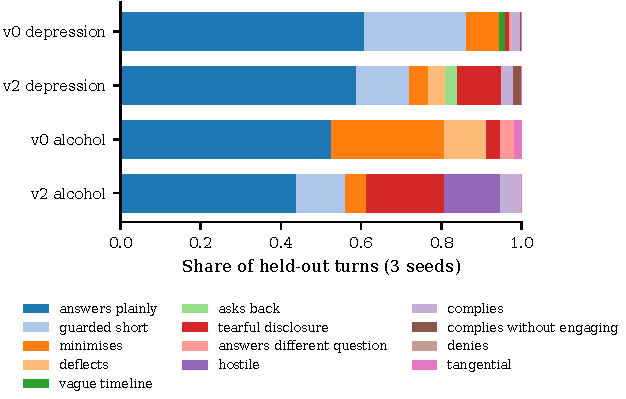
\includegraphics[width=\linewidth]{fig_behaviours.pdf}
\caption{How often each behaviour was used on held-out turns (three seeds).}
\label{p1:fig:behaviours}
\end{figure}

\begin{figure}[htbp]
\centering
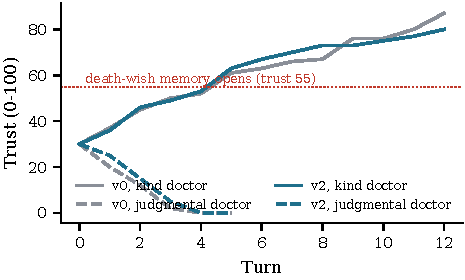
\includegraphics[width=\linewidth]{fig_trust.pdf}
\caption{Trust over a kind and a judgmental conversation (depression case, seed 11).}
\label{p1:fig:trust}
\end{figure}

\begin{figure}[htbp]
\centering
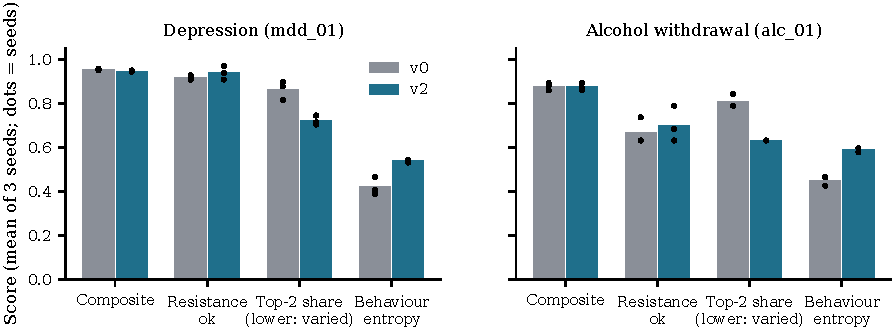
\includegraphics[width=\textwidth]{fig_heldout.pdf}
\caption{Held-out scores, v0 against v2 (bars: average of three seeds; dots: each seed). Accuracy (composite) is unchanged; resistance fits
the situation slightly better, and v2 spreads its behaviour over more kinds across conversations.}
\label{p1:fig:heldout}
\end{figure}

\begin{figure}[htbp]
\centering
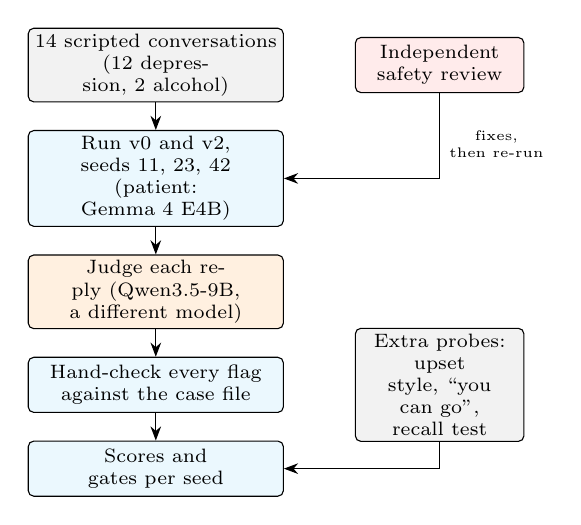
\begin{tikzpicture}[node distance=3.5mm]
\tikzset{b/.style={box=#1, text width=31mm}}
\node[b=gray!10] (a) {14 scripted conversations\\(12 depression, 2 alcohol)};
\node[b=cyan!8, below=of a] (b) {Run v0 and v2, seeds 11, 23, 42\\(patient: Gemma 4 E4B)};
\node[b=orange!12, below=of b] (c) {Judge each reply (Qwen3.5-9B,\\a different model)};
\node[b=cyan!8, below=of c] (d) {Hand-check every flag\\against the case file};
\node[b=cyan!8, below=of d] (e) {Scores and gates per seed};
\node[b=red!8, text width=20mm, right=9mm of a] (f) {Independent\\safety review};
\node[b=gray!10, text width=20mm, right=9mm of d] (g) {Extra probes:\\upset style, ``you\\can go'', recall test};
\draw[->] (a) -- (b); \draw[->] (b) -- (c); \draw[->] (c) -- (d); \draw[->] (d) -- (e);
\draw[->] (f.south) |- node[lab, right, pos=0.3]{fixes,\\then re-run} (b.east);
\draw[->] (g.south) |- (e.east);
\end{tikzpicture}
\caption{How v2 was validated.}
\label{p1:fig:protocol}
\end{figure}

\bibliographystyle{unsrt}
\bibliography{../shared/refs}
\end{document}
